
While the previous experiments demonstrate the potential benefits of unevenly setting up
the power caps and the number of active cores per socket in a power-constrained NUMA node,
these benefits are obtained under the huge cost of running each application multiple times
in the targeted NUMA node, each time with a particular power and active cores limit.
Further, the results obtained using extensive search on a particular NUMA node are not
applicable to another one since the hardware response to low power bounds are driven by
manufacturing variability and cannot be known in advance.  Also, deriving a particular
performance ratio per power bound among the sockets contained in a NUMA node is not enough
as different applications react in a different way to such variability.  It is thus
necessary to develop techniques able to quickly determine the optimal power-\# of cores
distribution for a particular software component and NUMA node.

We implement our method at the runtime level, since such systems offer load-balancing and
can be easily extended with additional functionality.  They are also widely used and
expected to play a significant role in future parallel architectures \cite{JSFI19,
Casas2015}. 


\subsection{Exploiting Application Structure}
Parallel codes often decompose loops or segments of serial code into multiple work units
that run in parallel.  While (at least to date) many codes follow the Single Program
Multiple Data (SPMD) approach where multiple cores execute the same code several times,
even more complex patterns, different repetitions of loops that iterate over similar sets
of data several times produce similar execution patterns.  As a consequence, codes almost
always exhibit a certain degree of repetitive behavior that can be observed either over
time or by considering the logical execution structure, which is composed of event
sequences~\cite{Isaacs2015, Totoni2014, Casas2010}.  This iterative nature of parallel
applications allows us to effectively guide the whole application behavior by observing
only small but significant portions of the parallel execution.  Our approach considers
execution segments and associates each with a particular power and number of active core
assignation per socket. To identify such a segment, the runtime tracks and identifies task
instances of the same task type. 
The intuition behind our approach is that same type tasks should behave in similar
fashion.   However, if tasks of the same type behave in an non-deterministic manner,
then our approach will fail to find a better configuration.
For example, in the case of \textit{blackscholes} we only
have one task type, thus this case is trivial.  However, in other applications, such as
\textit{ferret}, there are a few different task types.  For \textit{ferret} these are
\textit{t\_seg}, \textit{t\_extract}, \textit{t\_vec}, \textit{t\_rank} and
\textit{t\_out}.  The runtime can identify the type of an instance by the call site of the
taskified functions or user provided labels. Then, for a given monitoring window, the
runtime will identify all the task types running, but compare the execution time of the
tasks with the same type.  There are cases however that this may not be possible.  For
example if no tasks of the same type are found running on both sockets or if the tasks
of the same type run different workloads (their execution time varies beyond a
threshold, thus they  are not comparable), 
then the current monitoring window is discarded and move to the next
configuration.  This may cause the runtime to miss a good configuration, or even the
optimal one.
\par
Identifying representative segments of an application has been extensively studied, 
especially in the context of hardware simulation, where running the entire 
application is too slow.  Techniques such as the one presented by Sherwood et. al
\cite{Sherwood:2001:BBD:645988.674158} and the SimPoint 3.0 framework \cite{simpoints3}
could be employed for a more robust analysis and deal with the aforementioned issues. 
However, our approach exploits information already available to the runtime that can be 
accessed fast, minimizing the analysis' overhead. 
%makes it possible to
%explore many different configurations on representatives code sections in a single run,
%which can the be used in an online search.

\subsection{Search Algorithm}
\label{sec:algorithm}
The search algorithm aims to find the optimal power and total number of active cores
balance among the different sockets of a NUMA node.  It starts with evenly distributing
power and activating all cores and then progressively iterates over a set of power/\#cores
configurations and selects the best one.  Per each configuration, the targeted application
runs for a certain amount of time.  The particular amount of time each configuration runs
for is a parameter we call \textit{monitoring window}.  The smaller this parameter, the
shorter the exploration, but  the more chances of getting a non-optimal configuration
since the amount of time it has been trained for may not be representative of the whole
execution.  On the other hand, large window sizes significantly increase the chance of
finding the right configuration, but make the algorithmic search phase larger.

To characterize the performance achieved by each configuration we use a \textit{throughput
metric} defined as the number of tasks executed during the monitoring window each
configuration runs for.  This metric is well defined for all applications we consider in
this work (see Section~\ref{sec:setup}) and is particularly well-suited since it also
implicitly captures the amount of idle time spent by the active cores.  Further, it does
not imply a significant amount of measurement overhead if the task granularity is kept
over the tens of $\mu s$ threshold.  Although this metric is specific for task-based
codes, any other light-weight metric able to capture the amount of time spent doing useful
work would provide similar results for other kinds of applications or programming models.

During the first monitoring window, the runtime system measures the throughput of evenly
distributing power among the sockets and using all the available cores.  This is
considered the best candidate until a configuration providing larger throughput is
observed.  After each iteration we then compare the throughput for the current profile
with the best one.  If the current one is better, it becomes the new best and is used for
the subsequent comparisons.  This analysis continues until the search space is exhausted,
which may require more than one application run.  At the end of each run, if we have not
yet exhausted the search space, the runtime saves a checkpoint of the analysis state and
resumes it in a succeeding run.

Special care must be taken to make sure that we are considering monitoring windows that
constitute representative execution segments.  If two windows capture different task types
comparing them is not fair since different tasks have different execution times.  To
address this issue, we keep a set of task types for each different window.  If the task
sets collected during the best and current windows are not equal, it could mean that the
two configurations were run at a different stages of the application's execution.  We call
these incompatible profile results \textit{mismatching windows}.  When this occurs, we
ignore the current configuration without comparing it to the best and continue by checking
another configuration over the next monitoring window.  Special care need to be taken for
the first monitoring window.  If the first and second windows mismatch, we discard both
and retrain the first configuration.  This will continue until we capture a representative
segment of the application, meaning that two consecutive windows will be matching.

Note that different alternatives are available when dealing with mismatching windows.
However, for this work we employ the simplest case, which is to discard it.

 
\begin{figure*}[t]
        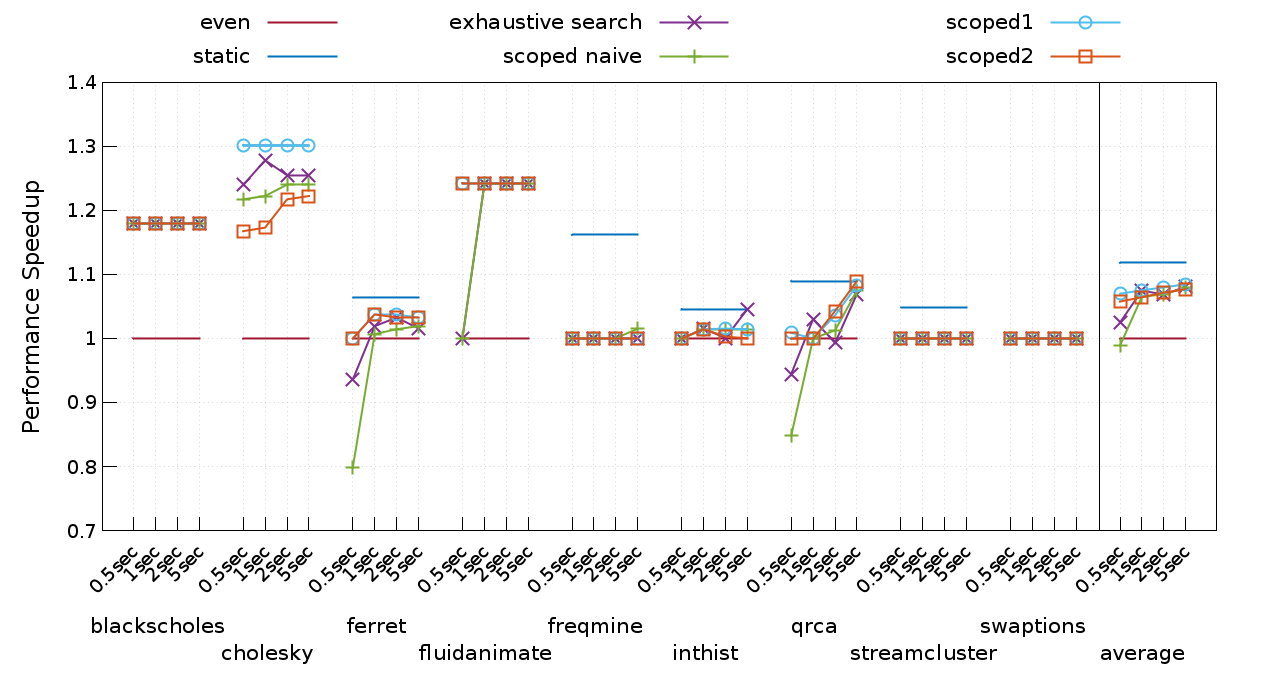
\includegraphics[width=\textwidth]{power_aware_runtime/figures/dynamic_window_impact}
        \caption{Comparison of best configuration found by exhaustive and scoped online analyses for different \textit{monitoring window} size, when running under a 80W power constraint.
                        The size of the monitoring window can influence the precision of the analysis.}
        \label{fig:mon_win_size_impact}%
\vspace{.5cm}
\end{figure*}



The search algorithm looks for the best configuration after trying several ones and
measuring their throughput over their corresponding monitoring windows.  As explained, the
monitoring windows size is an input parameter of our search algorithm.  The algorithm's
sensitivity to the windows size and its optimal value are explored in detail in
Section~\ref{sec:window_size_impact}.  Also, the set of configurations the search
algorithm iterates over is a key choice.  Large sets increase the chances of getting the
optimal power/\#active cores balance per socket, but also increases the cost of running
the search.  Alternatively, reduced sets may produce cheaper searches but also be unable
to find configurations that significantly improve performance. 

\subsection{Training Sets}
\label{sec:searchspaces}
We have implemented four variations of our analysis, based on the size of the configurations sets:

\textbf{Exhaustive Search:} We use the different configurations defined in
Section~\ref{sec:setup}.  As discussed above, in case we target a 80W power bound, the
exhaustive search considers 180 different configurations.  This is a conservative, but
expensive analysis. 


\textbf{Naive Scoped Search:} The scoped search does not consider extremely unbalanced
configurations since they rarely produce the most optimal results.  As a general rule we
focus the search on a small area around the default balanced configuration.  The reasoning
here is that just slightly providing more power or reducing the concurrency in the slower
socket will mitigate the imbalance between the sockets.  The scoped search considers 80
different configurations for the 80W bound.  They are composed of five different power
configurations (30W:50W, 35W:45W, 40W:40W, 45W:35W and 50W:30W) deployed for each one of
the 16 active core distributions: 6-6, 6-8, 6-10, 6-12, 8-6, ... , 12-12.

\textbf{Scoped Search 1:}
This training set aims to further reduce the search space, but considers both balanced and
unbalanced configurations.  It avoids irrational distributions like assigning more than
half of the power but less than half of the active cores to one of the sockets.  This
training set considers the even power configuration (40W:40W) and 9 different active cores
distributions for it: 8-8, 8-10, 8-12, 8-10, 10-10, 12-10, 8-12, 10-12 and 12-12.  It also
takes into account assigning 35W to the first socket and 45W to the second one with active
core counts 6-10, 6-12, 8-10 and 8-12 and its counterpart, that is, 45W to the first
socket and 35W to the second with active cores counts of 10-6, 12-6, 10-8 and 12-8.
Finally, this training set considers two unbalanced configurations: 30W:50W assigned to
the sockets and 2-12 active core counts per socket, and 50W:30W with 12-2 active cores.
This leaves us with 19 configurations when operating under the 80W power bound.

\textbf{Scoped Search 2:}
This training set contains the same distributions as Scoped Search 1 except the two
unbalanced configurations 50W:30W and 30W:50W, reducing the set to 17 configurations.
Very unbalanced configurations can produce large performance improvements, but also
increase the search costs since they significantly slowdown the execution in certain
cases.  This training set avoids the dangers of such unbalanced configurations by not
considering them. 

The reasoning here is that extreme configurations that greatly favor one socket or
severely reduce available parallelism are not likely to benefit an application.  Our goal
is to reduce the effect of the frequency imbalance between the sockets on a node, extreme
configurations would only benefit applications make sub-optimal use of the available
parallelism (e.g. dedup).

